\section{Técnicas de Clasificación}

Antes de empezar, y aunque no se ha implementado en la práctica, hacemos notar que por la descripción del problema parece que cometemos un error mayor cuando clasificamos mal la clase Yes. Por tanto, se podría considerar penalizar más los falsos negativos, de manera que los algoritmos de clasificación intenten cometer menores errores de este tipo. 

\subsection{Algoritmo KNN}

Recordamos los gráficos 1-1 con las clasificaciones, vistos en el EDA.

\vspace{\baselineskip}

\begin{figure}[H]\center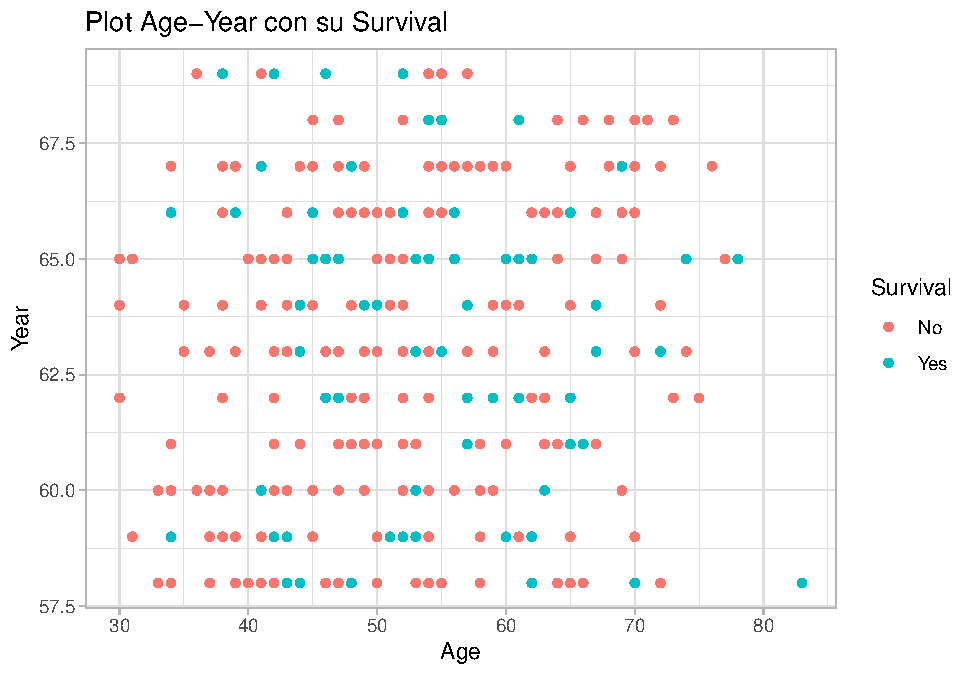
\includegraphics[width=.9\linewidth]{img/Clasificacion_files/figure-latex/unnamed-chunk-5-1}\caption{}\end{figure}

\begin{figure}[H]\center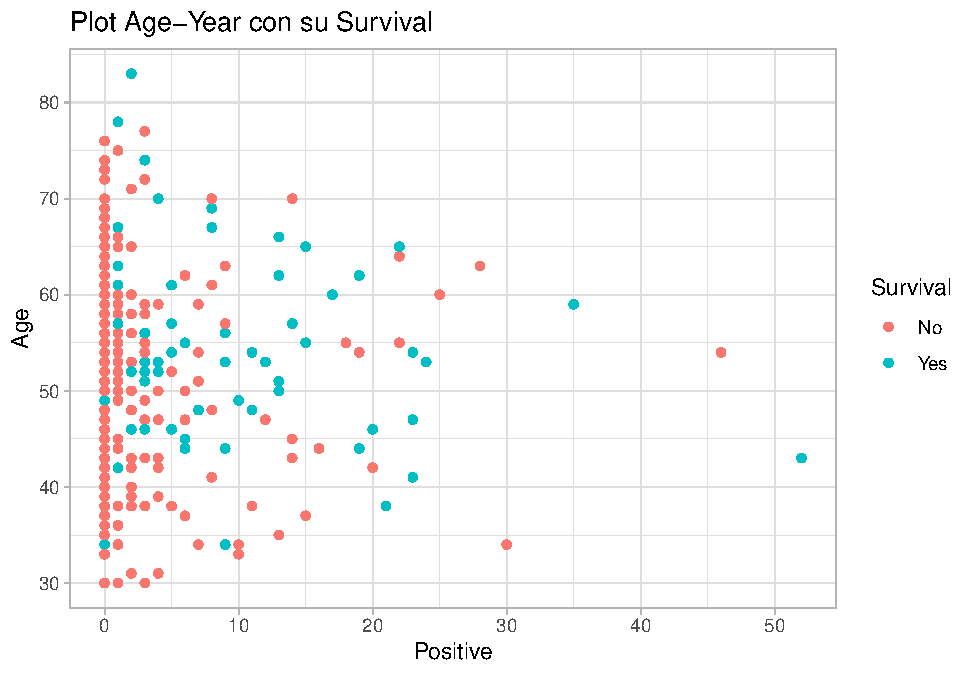
\includegraphics[width=.9\linewidth]{img/Clasificacion_files/figure-latex/unnamed-chunk-5-2}\caption{}\end{figure}

\begin{figure}[H]\center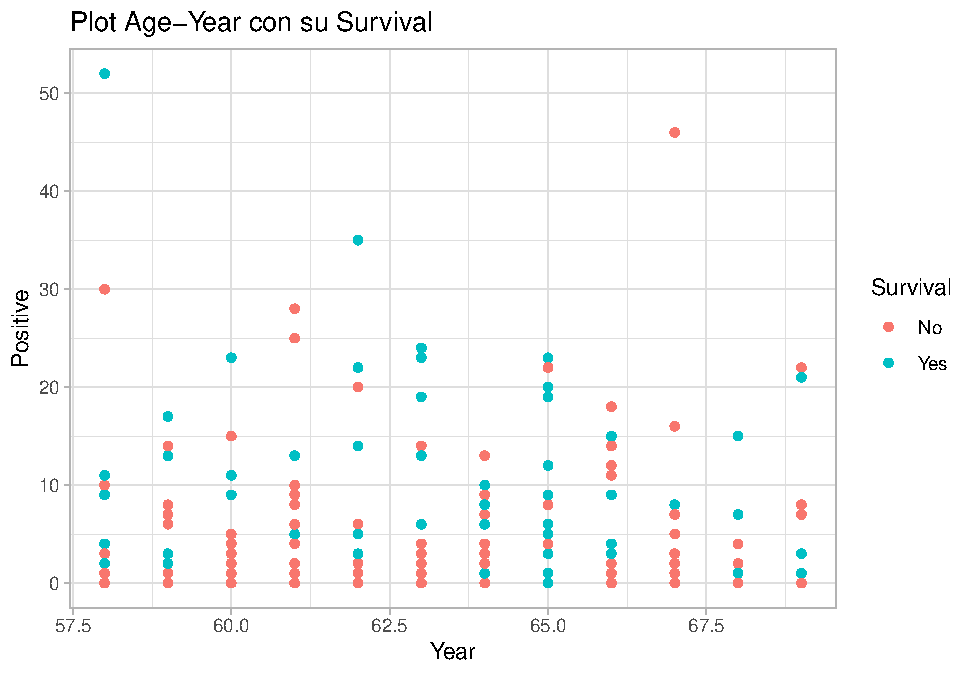
\includegraphics[width=.9\linewidth]{img/Clasificacion_files/figure-latex/unnamed-chunk-5-3}\caption{}\end{figure}

\begin{figure}[H]\center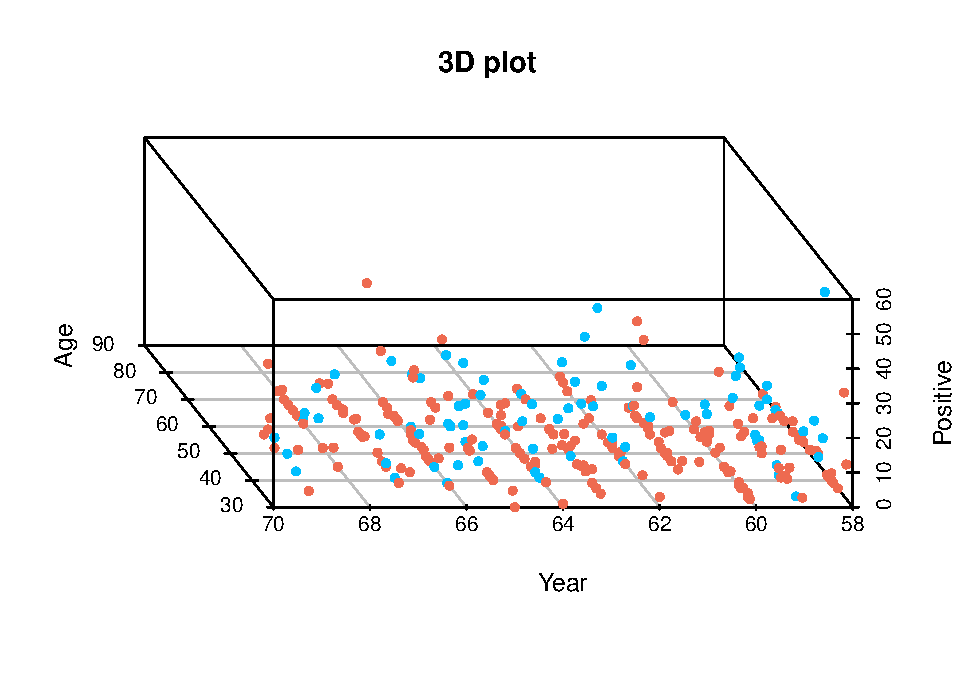
\includegraphics[width=.88\linewidth]{img/Clasificacion_files/figure-latex/unnamed-chunk-6-1}\caption{}\label{3d1}\end{figure}

\begin{figure}[H]\center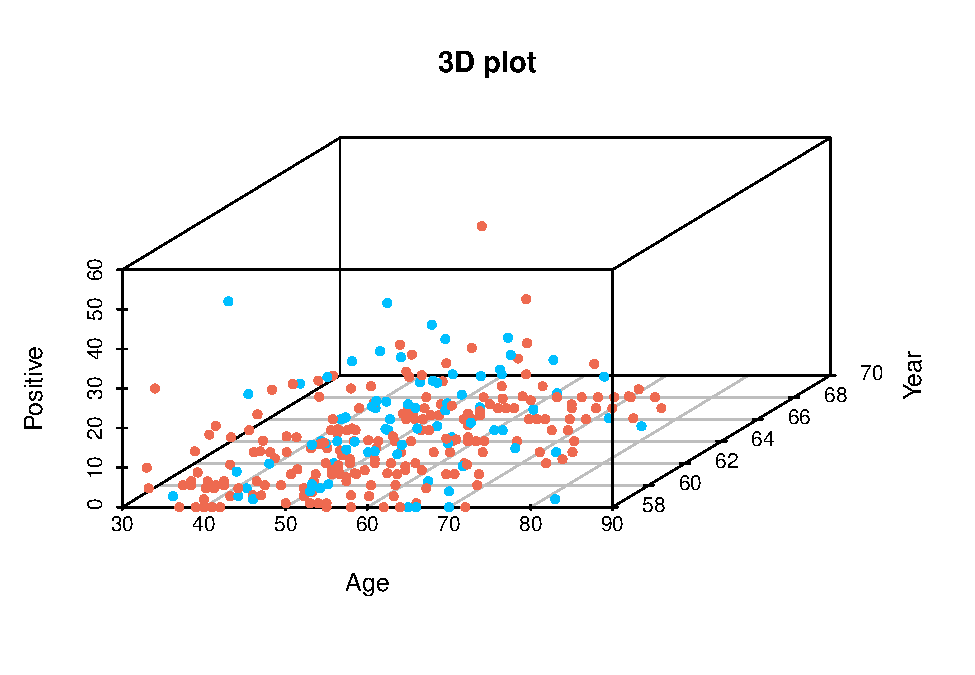
\includegraphics[width=.88\linewidth]{img/Clasificacion_files/figure-latex/unnamed-chunk-6-2}\caption{}\label{3d2}\end{figure}

De cara a un algoritmo KNN, apreciamos los datos muy entremezclados, con mayor tendencia a agruparse los no supervivientes (por su alta frecuencia) que los que sí, pero nada en especial que nos llame la atención.

Debido a esto vamos a empezar con un valor de K relativamente bajo y vamos a ir aumentándolo poco a poco. Tenemos que tener en cuenta que un K mayor puede ocasionar overfitting, pero usando técnicas de cross-validation podemos detectarlo con mayor facilidad.

\vspace{\baselineskip}

Los resultados usando el paquete caret son los siguientes\footnote{Los datos han sido preprocesados con una estandarización antes de aplicar cualquiera de los algoritmos de la práctica}:
\begin{verbatim}
k-Nearest Neighbors 

275 samples
  3 predictor
  2 classes: 'No', 'Yes' 

No pre-processing
Resampling: Cross-Validated (10 fold) 
Summary of sample sizes: 248, 248, 247, 247, 248, 247, ... 
Resampling results across tuning parameters:

  k   Accuracy   Kappa     
   3  0.6466931  0.05241865
   4  0.6612434  0.07153373
   5  0.6727513  0.05451908
   6  0.6907407  0.08157828
   7  0.6907407  0.07832535
   8  0.7017196  0.08311583
   9  0.7164021  0.13328924
  10  0.7089947  0.12077424
  11  0.7236772  0.15850208
  12  0.7161376  0.14004893
  13  0.7269841  0.16958772
  14  0.7197090  0.14121236
  15  0.7271164  0.16518141

Accuracy was used to select the optimal model using the largest value.
The final value used for the model was k = 15.
\end{verbatim}

\vspace{\baselineskip}

Vemos que al estar los datos tan entremezclados ni siquiera con un K pequeño aprende bien, es ya con un K medianamente alto (= 15) donde obtiene mayor accuracy en training.

\vspace{\baselineskip}

Una vez más probablemente esto se deba a la gran mezcla de los datos, de forma que necesite la ``opinión'' de un gran número de vecinos para poder predecir con mayor confianza el nuevo valor.

% Un K pequeño probablemente haga que la inmensa mayoría de puntos que etiqueta \textit{Yes} se clasifiquen como \textit{No}, al estar bastante esparcidos por el espacio.

\begin{figure}[H]\center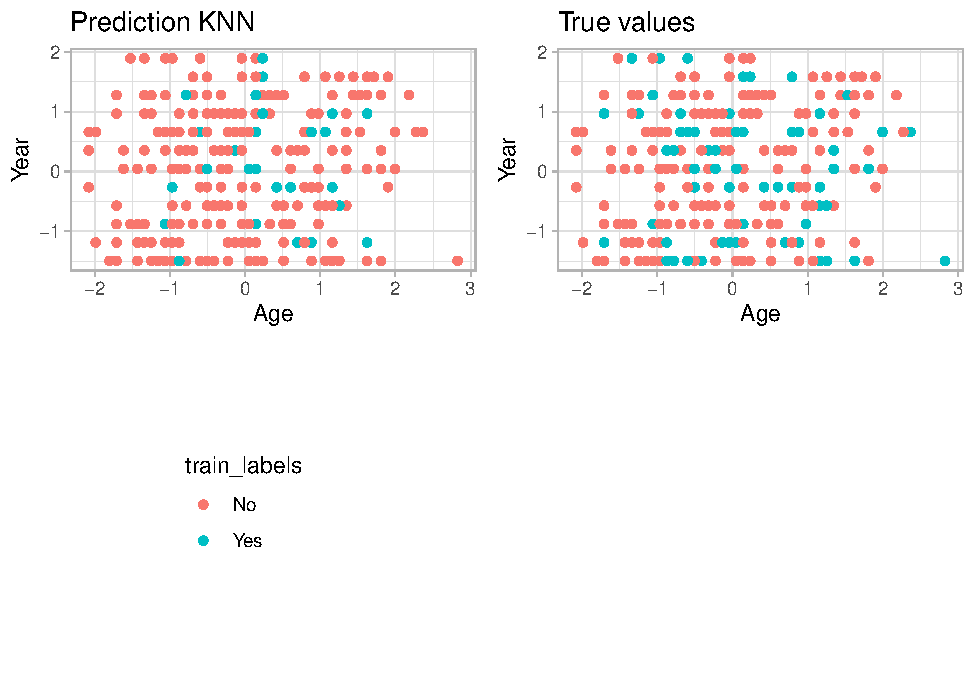
\includegraphics[width=.9\linewidth]{img/Clasificacion_files/figure-latex/unnamed-chunk-10-1}\caption{Predicción con K=15 en training}\end{figure}

Vemos que el uso de un K alto hace que perdamos puntos de Yes, puesto que no hay suficientes vecinos de la misma clase que refuercen la opinión sobre esa zona del espacio.

\vspace{\baselineskip}

Una evaluación con el subconjunto reservado inicialmente como test nos muestra una calidad extrañamente superior que la de training.

\begin{verbatim}
Test evaluation:
 Accuracy     Kappa 
0.8387097 0.2439024 

Confusion matrix (in test split):
knnPred No Yes
    No  25   5
    Yes  0   1


Etiquetas reales:
No  No  Yes No  No  No  Yes No  No  No  No  No  No  No  Yes No  No  Yes Yes
No  No  No  No  No  No  No  Yes No  No  No  No 

Predicciones KNN:
No  No  No  No  No  No  No  No  No  No  No  No  No  No  No  No  No  No  Yes
No  No  No  No  No  No  No  No  No  No  No  No 
\end{verbatim}

\begin{figure}[H]\center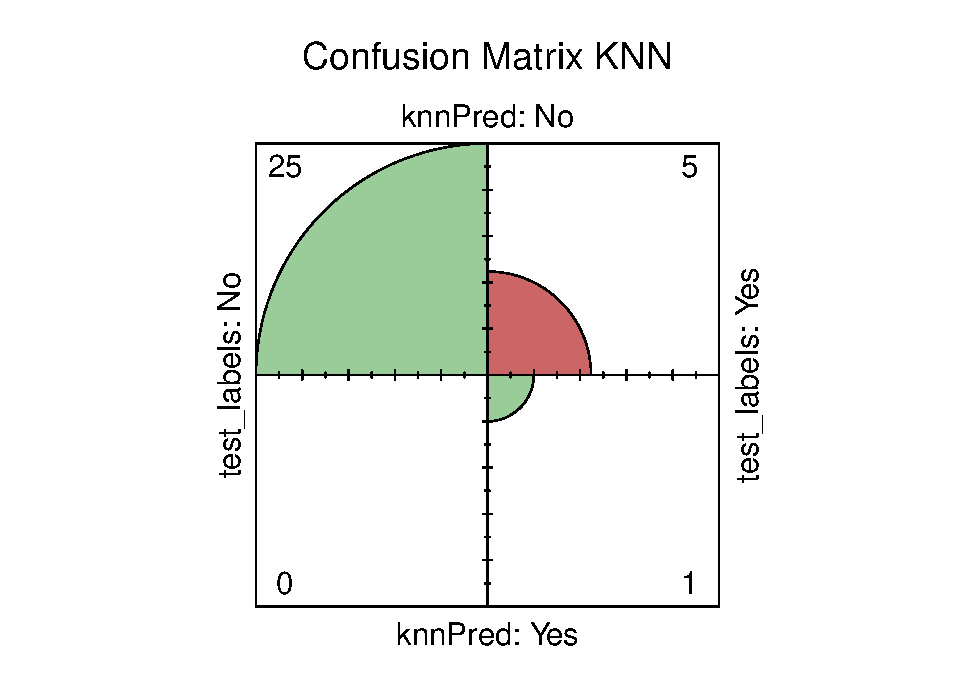
\includegraphics[width=.9\linewidth]{img/Clasificacion_files/figure-latex/unnamed-chunk-9-1}\caption{Matriz de confusión sobre el conjunto de test}\end{figure}

Este comportamiento no es el habitual en aprendizaje automático, parece que casualmente el conjunto de test es bastante fácil de ajustar y por eso se obtienen mejores resultados que en training.

\vspace{\baselineskip}

Vemos que no se produce ni un solo falso negativo en nuestro conjunto de test. El valor alto de K hace que se prediga con mayor facilidad este valor \textit{No} de etiqueta y por ese desbalanceo se obtengan tan buenos resultados.

\vspace{\baselineskip}

Si enfocamos el problema como una predicción no limitada al hospital y a los años de las muestras, este hecho es en sí es un poco preocupante, pues no sabemos si esta tendencia es constante en todos los pacientes. Pese a ello, debemos suponer que la muestra que tenemos es representativa y por tanto válida.

Por otro lado, como estamos tratando con un problema médico, esto quizás podría ser incluso un hecho positivo, ya que los falsos positivos sería algo que querríamos evitar a toda costa (todo depende del enfoque hacia el que se haya orientado el estudio).

\newpage

Por comparar, podemos también evaluar con otros valores de K en test. Puesto que hemos obtenido los mejores resultados en training con un K de 15, que es un valor relativamente alto, podemos probar con uno bajo y uno intermedio (3 y 7).

\begin{verbatim}
k-Nearest Neighbors

No pre-processing
Resampling: Cross-Validated (10 fold) 
Summary of sample sizes: 247, 248, 247, 248, 248, 247, ... 
Resampling results:

  Accuracy   Kappa     
  0.6654762  0.09645955

Tuning parameter 'k' was held constant at a value of 3
\end{verbatim}

\begin{verbatim}
Test evaluation:
Accuracy     Kappa 
0.8064516 0.2900763 

Confusion matrix (in test split):
         test_labels
knn3Pred   No Yes
       No  23   4
       Yes  2   2
\end{verbatim}

\begin{figure}[H]\center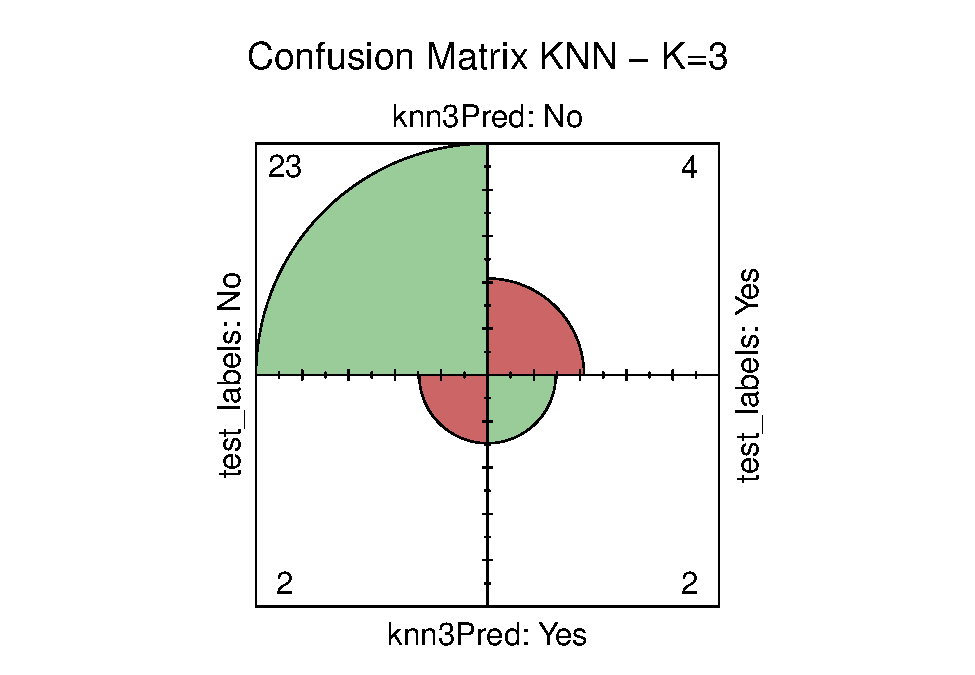
\includegraphics[width=.9\linewidth]{img/Clasificacion_files/figure-latex/unnamed-chunk-12-1}\caption{Matriz de confusión sobre el conjunto de test}\end{figure}

\newpage

\begin{verbatim}
k-Nearest Neighbors 

No pre-processing
Resampling: Cross-Validated (10 fold) 
Summary of sample sizes: 248, 247, 247, 248, 247, 247, ... 
Resampling results:

  Accuracy   Kappa     
  0.6874339  0.08134908

Tuning parameter 'k' was held constant at a value of 7
\end{verbatim}

\begin{verbatim}
Test evaluation:
Accuracy     Kappa 
0.8064516 0.1696429 

Confusion matrix (in test split):
        test_labels
knn7Pred No Yes
     No  24   5
     Yes  1   1
\end{verbatim}

\begin{figure}[H]\center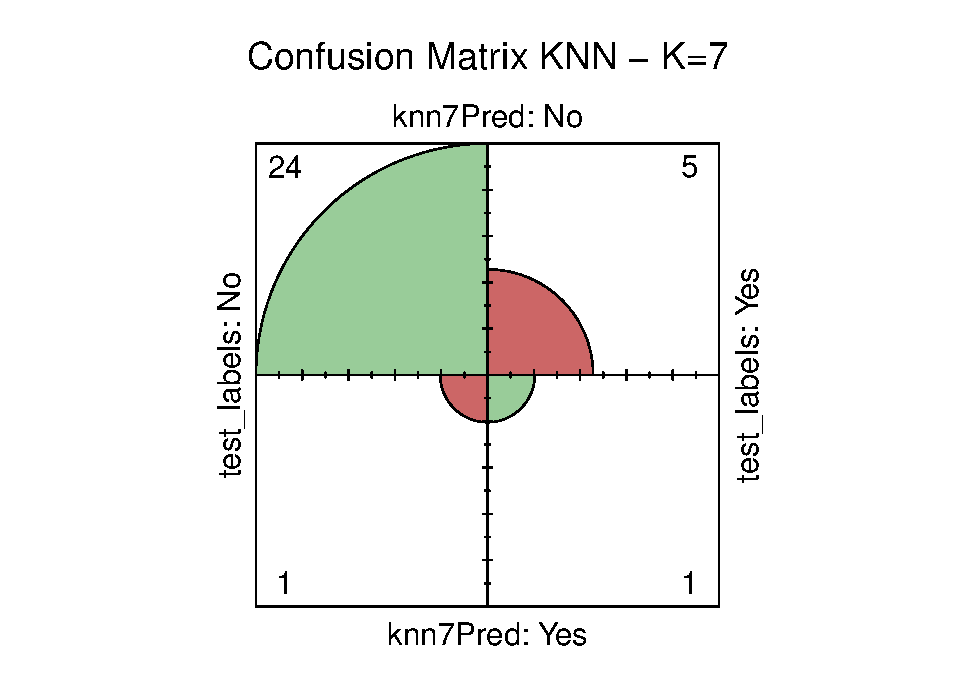
\includegraphics[width=.9\linewidth]{img/Clasificacion_files/figure-latex/unnamed-chunk-14-1}\caption{Matriz de confusión sobre el conjunto de test}\end{figure}

K=7 vemos que es el que más sufre al evaluar en test, y ambos (tal y como nos había indicado la primera ejecución con CV) tienen una calidad bastante inferior (tanto en training como en test) a un K=15.

\subsection{Algoritmo LDA}
\subsubsection{Asunciones}
Comprobamos asunciones:
\begin{enumerate}
    \item \textbf{Distribución aleatoria}: No nos queda más remedio que creer que sí.
    \item \textbf{Cada predictor sigue una distribución normal}: Ya vimos en el EDA que esto no era cierto. El test de Shapiro nos aseguraba que no había normalidad en ninguna de las variables y los QQ-plots nos lo hacían ver claramente. Técnicamente sabiendo esto no deberíamos usar LDA, pero puesto que esto es un proyecto seguimos.
    
    Por otro lado, las variables Age y Year no parecen seguir una distribución demasiado ``rara'' (en comparación con una normal), por lo que es posible que al menos obtengamos resultados de calidad aceptable.
    \item \textbf{Las clases siguen la misma matriz de covarianza}: Lo comprobamos a continuación.
\end{enumerate}

Calculamos la diagonal de la matriz de correlación para cada una de las clases, obteniendo:
\begin{verbatim}
Para clase Yes:
      Age      Year  Positive 
0.9439366 1.0656924 1.7401564 

Para clase No:
      Age      Year  Positive 
1.0423639 0.9998632 0.7266195 
\end{verbatim}

\vspace{\baselineskip}

Estos valores nos parecen indicar que al menos la variable Positive parece tener distintas varianzas, pero es preferible asegurarlo con un test estadístico.

Puesto que nuestras variables no siguen una distribución normal, no podemos hacer el test de homogeneidad de Barlett. Utilizamos por tanto el de Levene:
\begin{verbatim}
Age:
\end{verbatim}

\begin{tabular}{l|r|r|r}
\hline
  & Df & F value & Pr(>F)\\
\hline
group & 1 & 1.799898 & 0.1807261\\
\hline
 & 304 &  & \\
\hline
\end{tabular}

\begin{verbatim}
Year:
\end{verbatim}

\begin{tabular}{l|r|r|r}
\hline
  & Df & F value & Pr(>F)\\
\hline
group & 1 & 0.0624405 & 0.8028481\\
\hline
 & 304 &  & \\
\hline
\end{tabular}

\begin{verbatim}
Positive:
\end{verbatim}

\begin{tabular}{l|r|r|r}
\hline
  & Df & F value & Pr(>F)\\
\hline
group & 1 & 18.78912 & 1.99e-05\\
\hline
 & 304 &  & \\
\hline
\end{tabular}

Indicándonos que solo se puede asegurar que la variable Positive \textbf{no} tiene homogeneidad entre clases diferentes.

\vspace{\baselineskip}

Mostramos las distribuciones entre clases gráficamente:

\begin{figure}[H]\center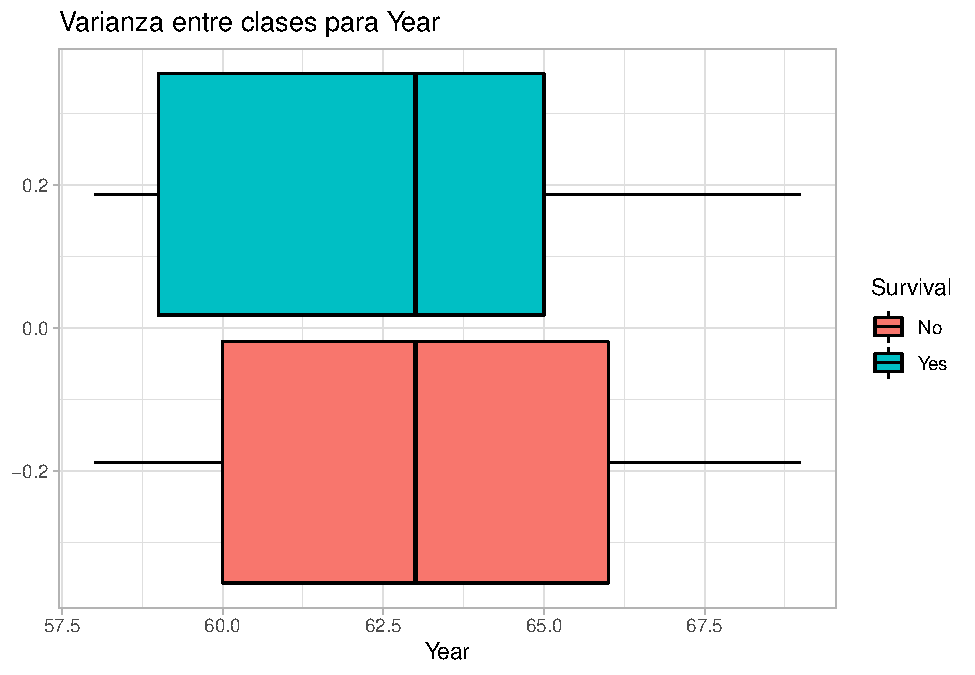
\includegraphics[width=.8\linewidth]{img/Clasificacion_files/figure-latex/unnamed-chunk-17-1}\caption{}\end{figure}

\begin{figure}[H]\center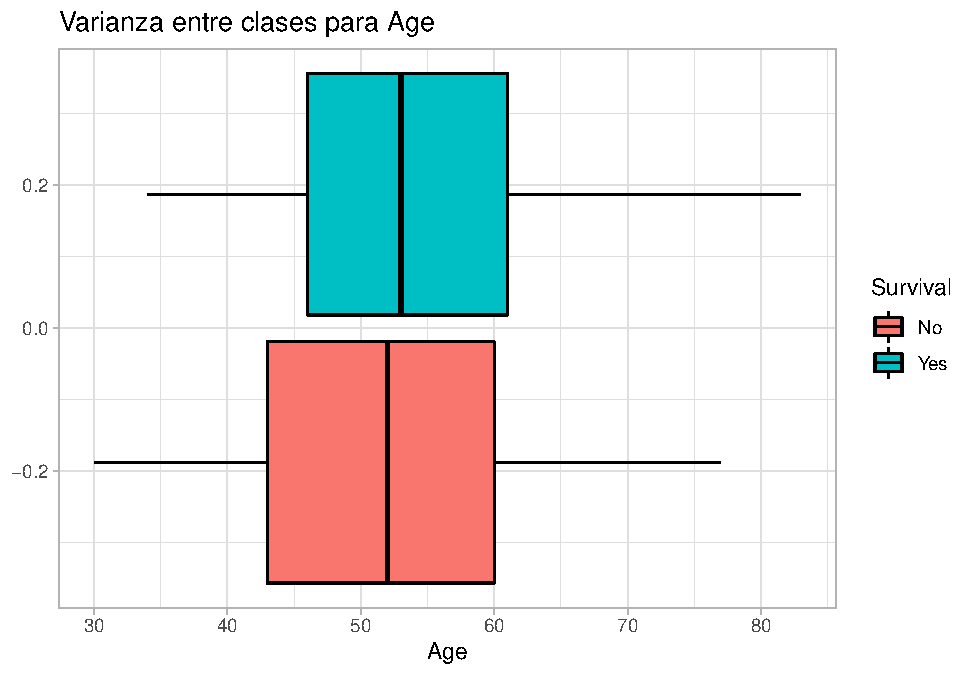
\includegraphics[width=.8\linewidth]{img/Clasificacion_files/figure-latex/unnamed-chunk-17-2}\caption{}\end{figure}

\begin{figure}[H]\center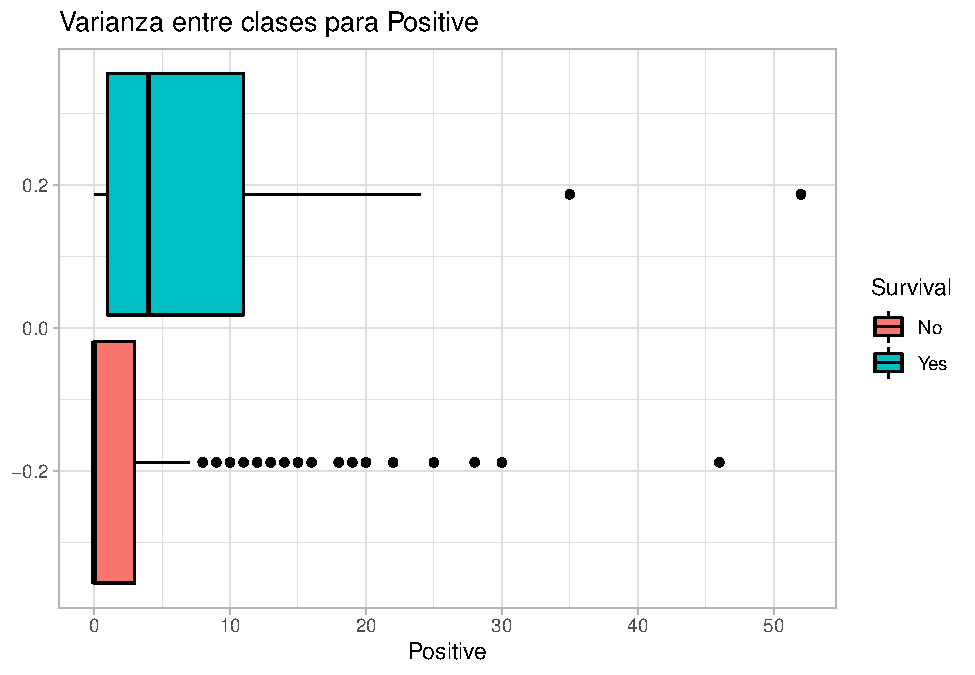
\includegraphics[width=.8\linewidth]{img/Clasificacion_files/figure-latex/unnamed-chunk-17-3}\caption{}\end{figure}

\begin{figure}[H]\center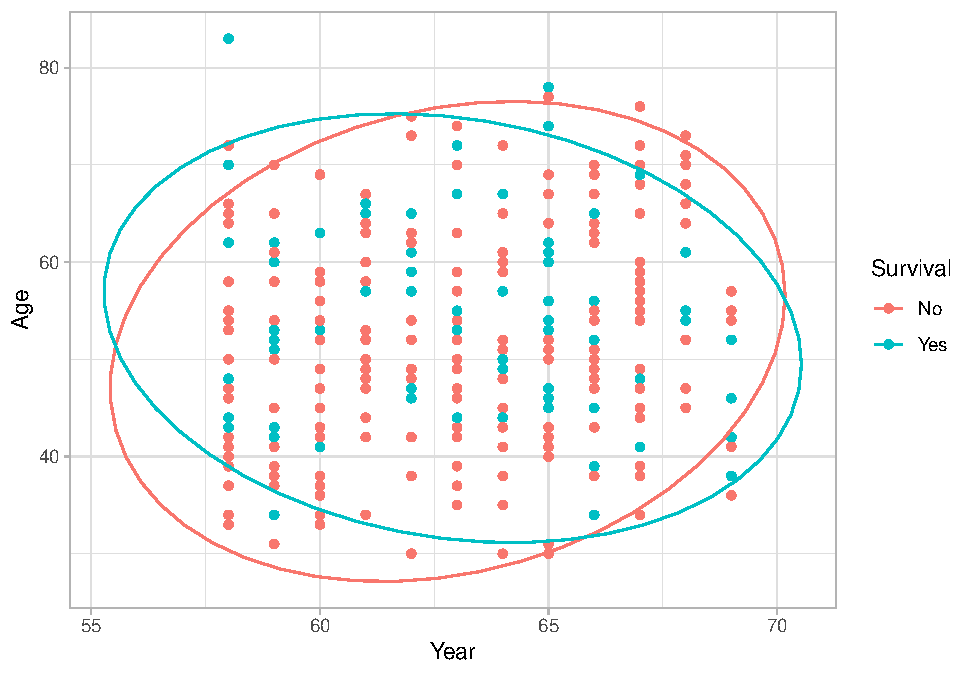
\includegraphics[width=.8\linewidth]{img/Clasificacion_files/figure-latex/unnamed-chunk-18-1}\caption{}\end{figure}

\begin{figure}[H]\center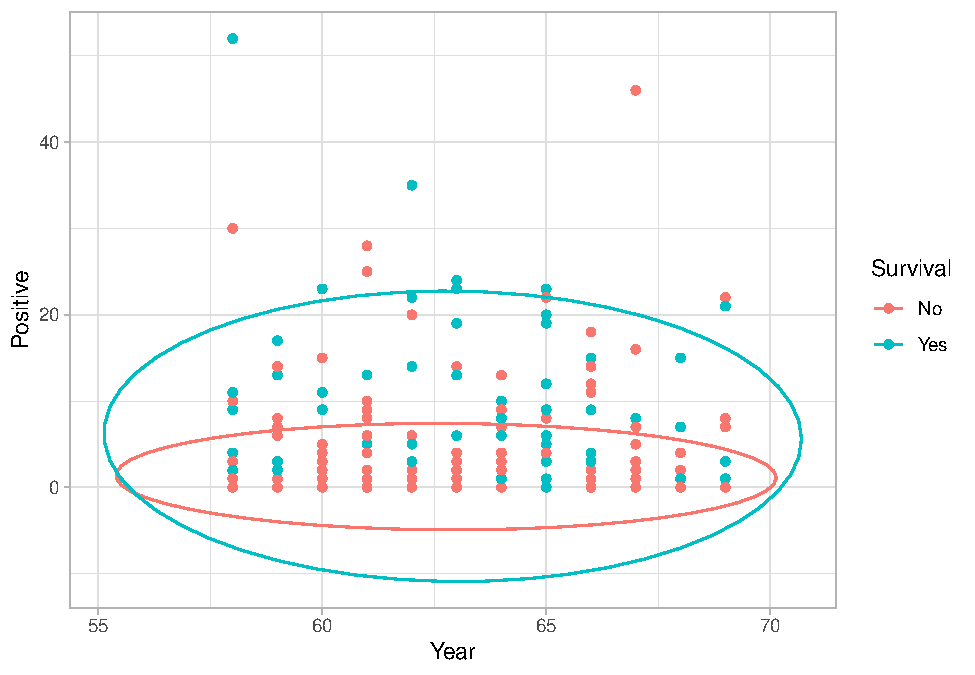
\includegraphics[width=.8\linewidth]{img/Clasificacion_files/figure-latex/unnamed-chunk-18-2}\caption{}\end{figure}

\begin{figure}[H]\center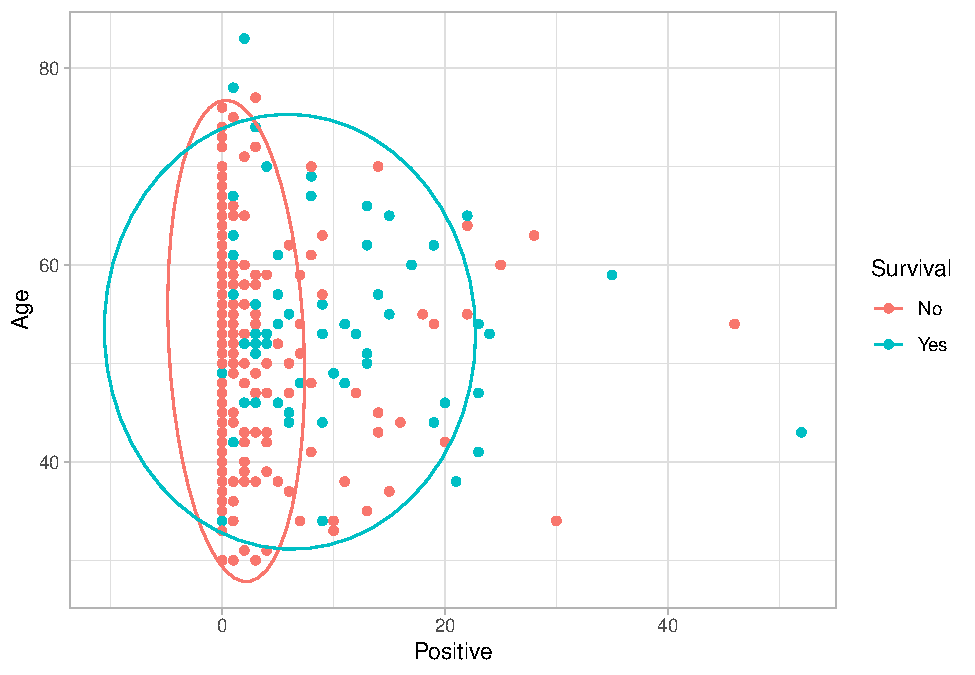
\includegraphics[width=.8\linewidth]{img/Clasificacion_files/figure-latex/unnamed-chunk-18-3}\caption{}\end{figure}

Se nota que la causa de que no se rechace el test para esta variable es la gran cantidad de datos con Positive igual a 0.

\vspace{\baselineskip}

Por tanto para LDA no podemos hacer uso de la variable Positive, puesto que además de la falta de normalidad se incumpliría la asunción número 3, por lo que haremos uso de las otras dos.

\vspace{\baselineskip}

Para terminar, aunque solo es recomendable y no son cualidades necesarias para obtener solución en LDA:
\begin{itemize}
    \item Tenemos más instancias que predictores, por varios órdenes de magnitud.
    \item Los predictores son independientes. 
    \item No tenemos varianzas cercanas a cero.
\end{itemize}

\subsubsection{Aplicación del algoritmo LDA}

\begin{verbatim}
Call:
lda(x, y)

Prior probabilities of groups:
       No       Yes 
0.7272727 0.2727273 

Group means:
            Age        Year
No  -0.05947324 -0.00398263
Yes  0.11192259 -0.03680916

Coefficients of linear discriminants:
            LD1
Age   0.9781149
Year -0.2588776
Cross-Validated (10 fold) Confusion Matrix 

(entries are percentual average cell counts across resamples)
 
          Reference
Prediction   No  Yes
       No  72.7 27.3
       Yes  0.0  0.0
                            
 Accuracy (average) : 0.7273
\end{verbatim}

\begin{figure}[H]\center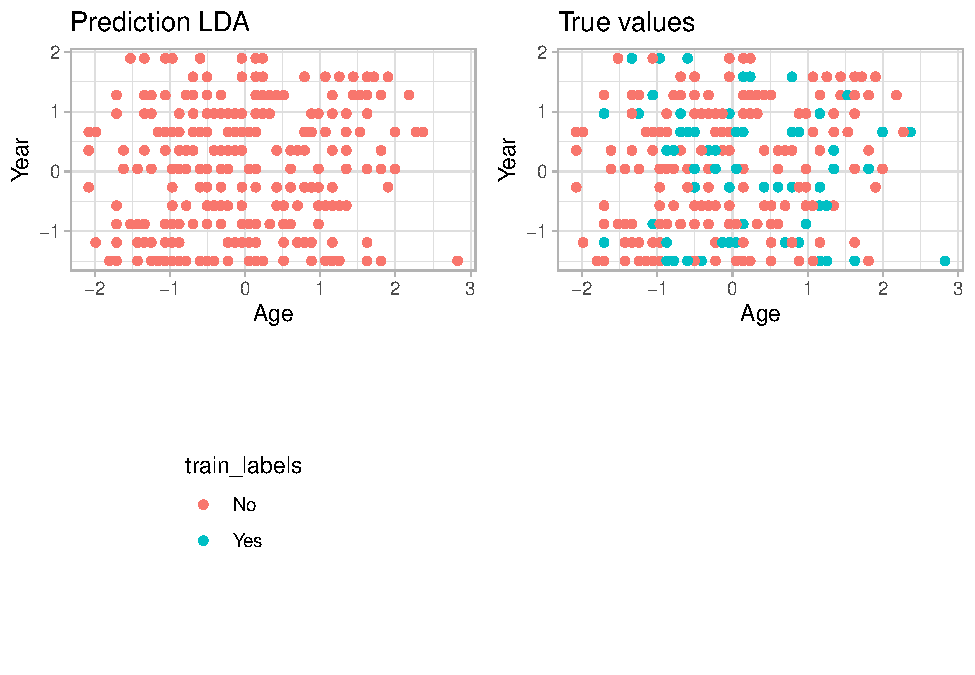
\includegraphics[width=.9\linewidth]{img/Clasificacion_files/figure-latex/unnamed-chunk-22-1}\caption{Predicciones LDA sobre training}\end{figure}

El gráfico de los discriminantes no muestra una buena separación entre las clases, estando ambos centrados sobre 0.5 y similarmente esparcidos.
\begin{figure}[H]\center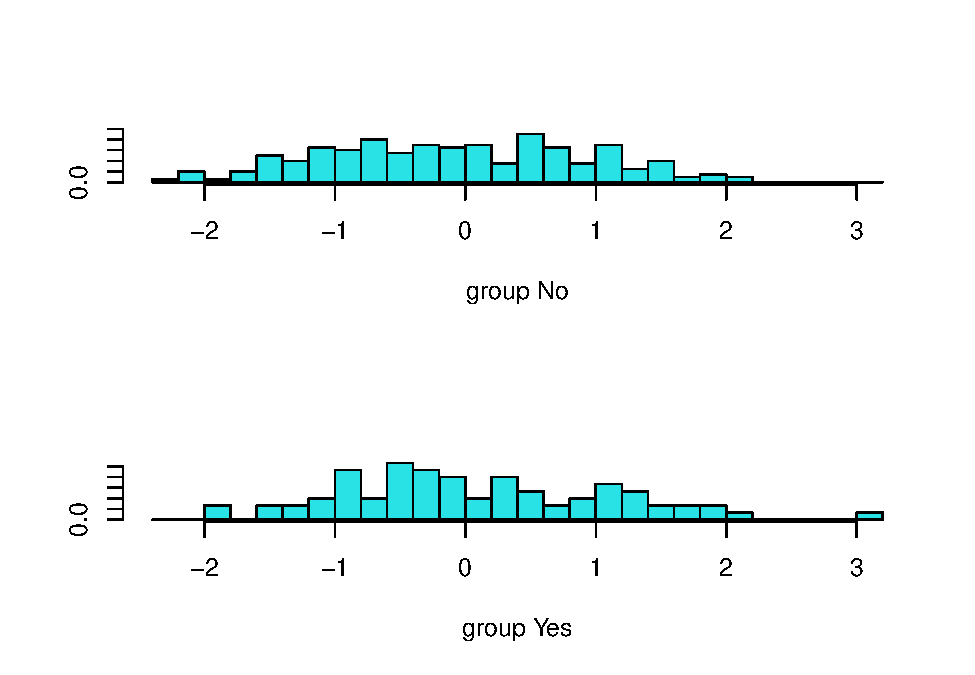
\includegraphics[width=.9\linewidth]{img/Clasificacion_files/figure-latex/unnamed-chunk-23-1}\caption{Histograma de los coeficientes de LDA}\end{figure}

Y aunque es difícil verlo en 2D, se puede apreciar que el hiperplano que se genera con LDA no separa bien las clases:
\begin{figure}[H]\center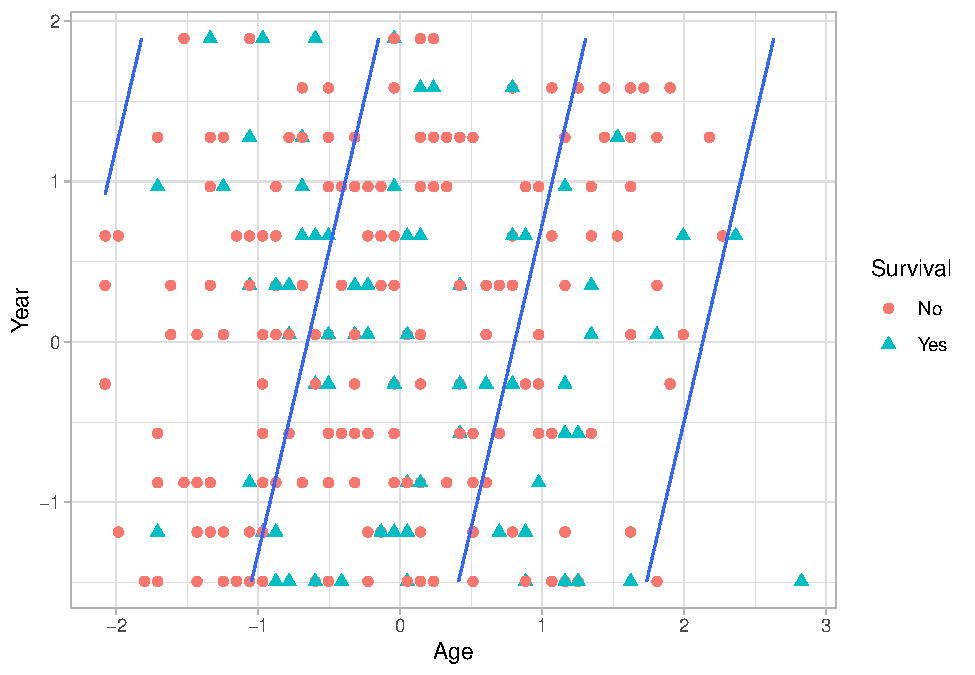
\includegraphics[width=.9\linewidth]{img/Clasificacion_files/figure-latex/unnamed-chunk-24-1}\caption{}\small{Estamos pintando un contorno 3D y por eso nos salen múltiples líneas en el gráfico}\end{figure}

\vspace{\baselineskip}

Resultados en test:
\begin{verbatim}
Test evaluation:
Accuracy     Kappa 
0.8064516 0.0000000

Confusion matrix (in test split):
       test_labels
ldaPred No Yes
    No  25   6
    Yes  0   0


Etiquetas:
No  No  Yes No  No  No  Yes No  No  No  No  No  No  No  Yes No  No  Yes Yes
No  No  No  No  No  No  No  Yes No  No  No  No 

Predicciones LDA:
No No No No No No No No No No No No No No No No No No No No No No No No No
No No No No No No
\end{verbatim}

\begin{figure}[H]\center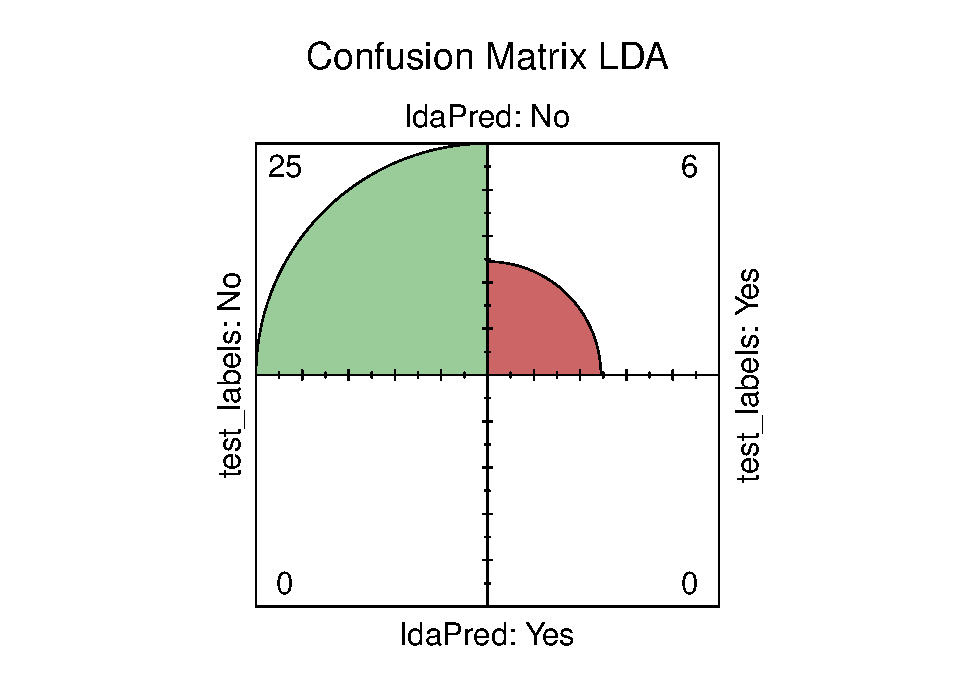
\includegraphics[width=.9\linewidth]{img/Clasificacion_files/figure-latex/unnamed-chunk-21-1}\caption{Matriz de confusión sobre el conjunto de test}\end{figure}

Tenemos un dataset bastante desbalanceado, y al menos con nuestros datos LDA no predice para la clase Yes. Con esto se asegura un alto accuracy en nuestro entrenamiento, pero está claro que este comportamiento lo vuelve un mal modelo en este problema, ya que (en base únicamente a las predicciones) no parece que haya aprendizaje.

\vspace{\baselineskip}

Adicionalmente los resultados en test nos devuelven un kappa igual a cero, dándonos a entender que estos son poco fiables y que se podría obtener esa misma calidad con aleatoriedad pura.

\newpage

\subsection{Algoritmo QDA}
\subsubsection{Asunciones}

QDA tiene las mismas asunciones de LDA salvo que relaja la necesidad de que para una variable las clases tengan igual covarianza. Esto nos permite usar la variable Positive que habíamos descartado en LDA.

\vspace{\baselineskip}

Por tanto, nos quedan los requisitos de: 
\begin{enumerate}
    \item \textbf{Distribución aleatoria}: Dábamos por hecho que sí.
    \item \textbf{Distribución normal}: No la tenía ninguna variable.
\end{enumerate}

Donde técnicamente el no cumplir normalidad no imposibilita que se encuentre solución, pero ya no nos lo asegura.

\vspace{\baselineskip}
\vspace{\baselineskip}

Y adicionalmente tenemos de forma recomendada que: 
\begin{itemize}
  \item \textbf{El número de predictores debe ser menor que el número de instancias de cada clase}: Del EDA sabemos que esto es cierto.
  \item \textbf{Los predictores dentro de cada clase no deben estar correlacionados}: Corroboramos que no se da en las siguientes matrices de correlación.
\end{itemize}

\vspace{\baselineskip}

\begin{figure}[H]\center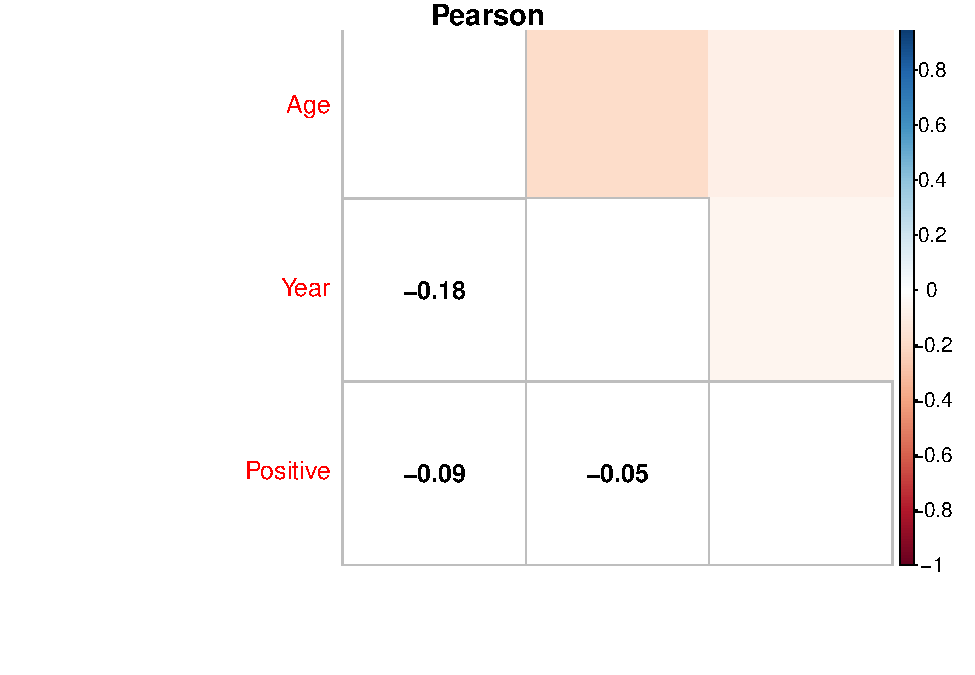
\includegraphics[width=.9\linewidth]{img/Clasificacion_files/figure-latex/unnamed-chunk-25-1}\caption{Matriz de correlación para la clase \textit{Yes}}\end{figure}

\begin{figure}[H]\center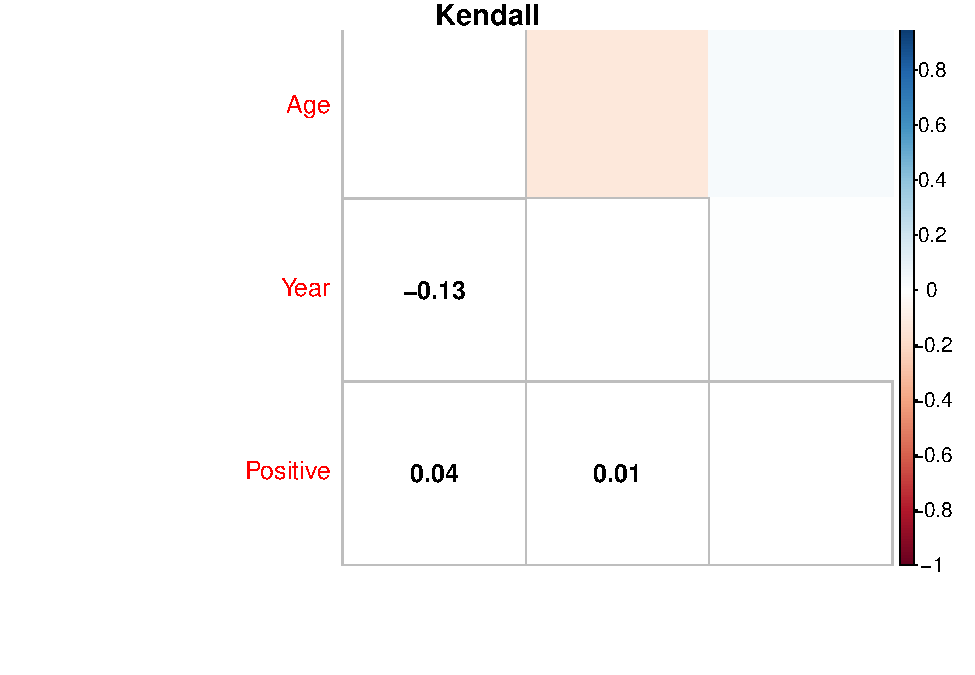
\includegraphics[width=.9\linewidth]{img/Clasificacion_files/figure-latex/unnamed-chunk-25-2}\caption{Matriz de correlación para la clase \textit{Yes}}\end{figure}

\begin{figure}[H]\center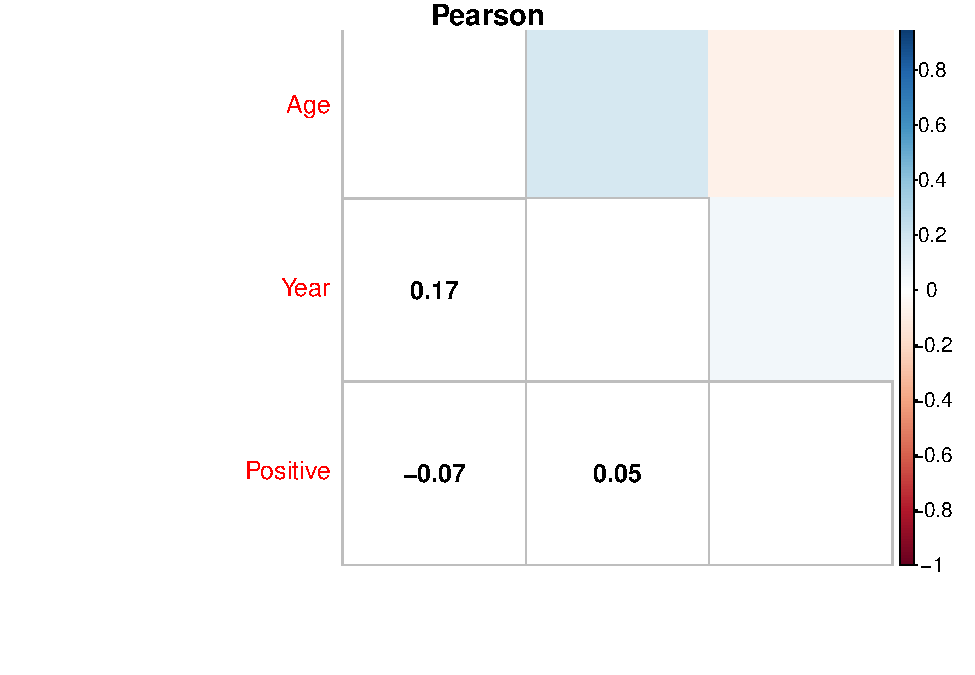
\includegraphics[width=.9\linewidth]{img/Clasificacion_files/figure-latex/unnamed-chunk-26-1}\caption{Matriz de correlación para la clase \textit{No}}\end{figure}

\begin{figure}[H]\center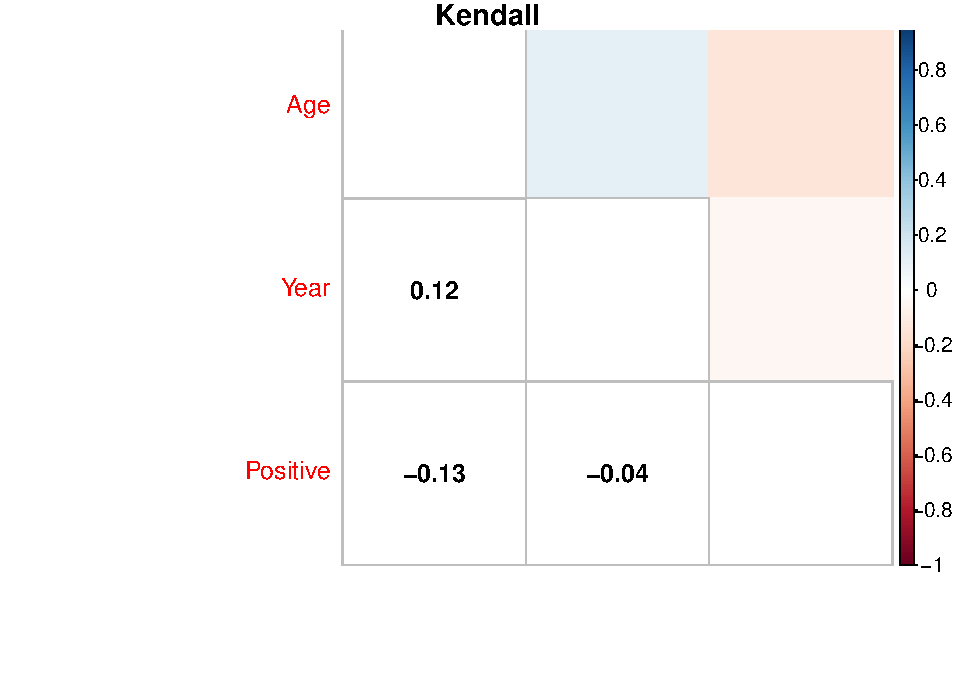
\includegraphics[width=.9\linewidth]{img/Clasificacion_files/figure-latex/unnamed-chunk-26-2}\caption{Matriz de correlación para la clase \textit{Yes}}\end{figure}

\subsubsection{Aplicación del algoritmo QDA}

\begin{verbatim}
Call:
qda(x, y)

Prior probabilities of groups:
       No       Yes 
0.7272727 0.2727273 

Group means:
            Age        Year   Positive
No  -0.05947324 -0.00398263 -0.1503750
Yes  0.11192259 -0.03680916  0.4933742
Cross-Validated (10 fold) Confusion Matrix 

(entries are percentual average cell counts across resamples)
 
          Reference
Prediction   No  Yes
       No  68.7 21.5
       Yes  4.0  5.8
                            
 Accuracy (average) : 0.7455
\end{verbatim}

\begin{figure}[H]\center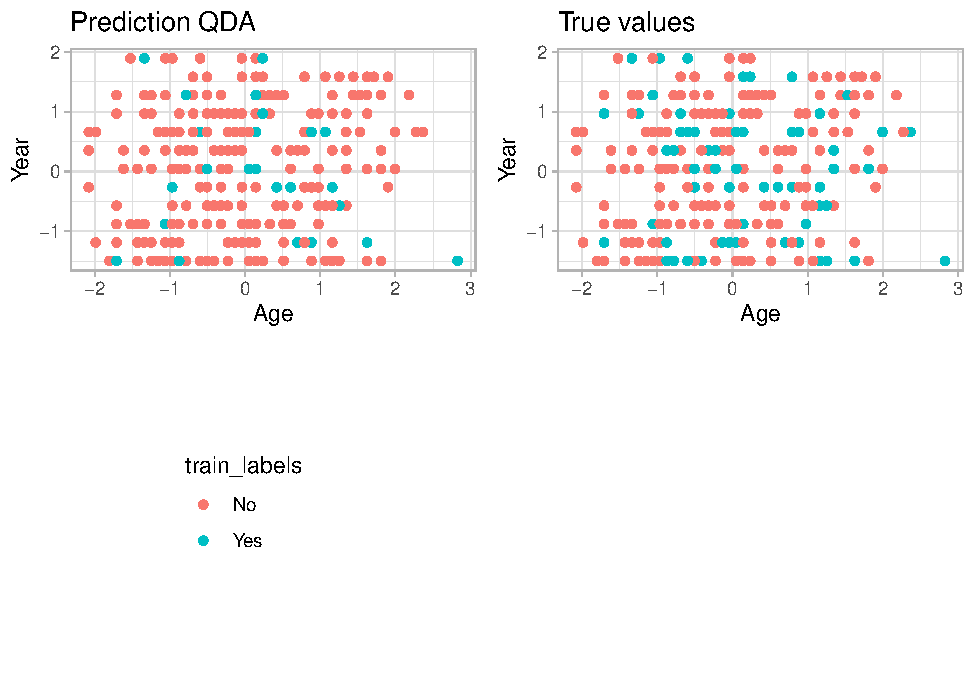
\includegraphics[width=.78\linewidth]{img/Clasificacion_files/figure-latex/unnamed-chunk-30-1}\caption{Predicciones QDA sobre training}\end{figure}

\vspace{\baselineskip}

\begin{verbatim}
Test evaluation:
Accuracy     Kappa 
0.8064516 0.0000000

Confusion matrix (in test split):
       test_labels
qdaPred No Yes
    No  25   6
    Yes  0   0



Etiquetas:
No  No  Yes No  No  No  Yes No  No  No  No  No  No  No  Yes No  No  Yes Yes
No  No  No  No  No  No  No  Yes No  No  No  No 

Predicciones QDA:
No No No No No No No No No No No No No No No No No No No No No No No No No
No No No No No No
\end{verbatim}

\begin{figure}[H]\center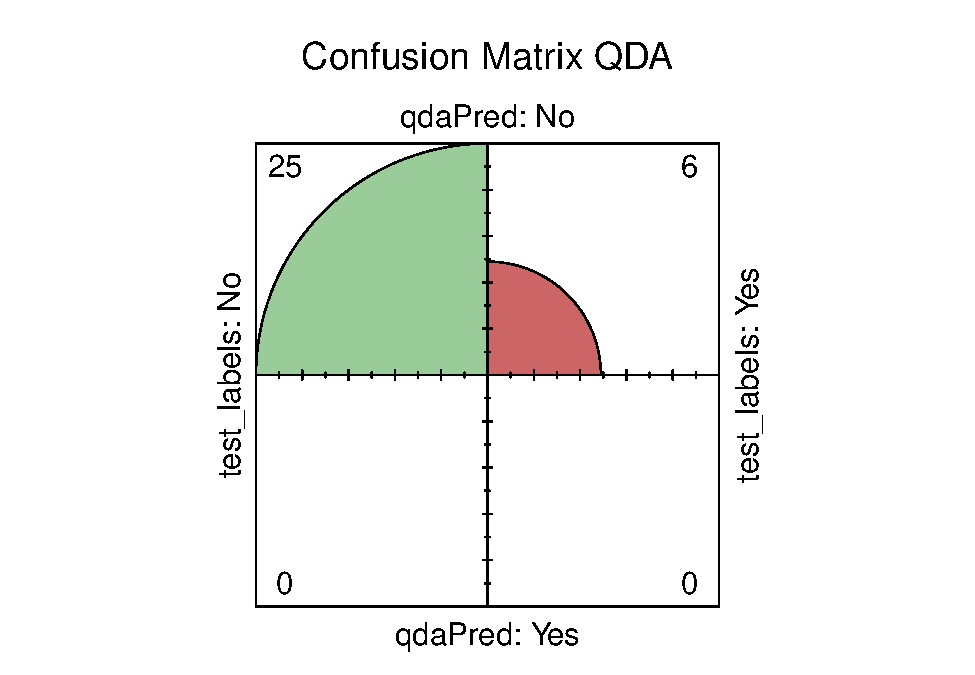
\includegraphics[width=\linewidth]{img/Clasificacion_files/figure-latex/unnamed-chunk-29-1}\caption{Matriz de confusión sobre el conjunto de test}\end{figure}

Obtenemos los mismos resultados en test que LDA, pero en este caso vemos que sobre training sí se predice la clase \textit{Yes}. Por tanto, podemos suponer que el hiperplano que forma no es tan restrictivo como el de LDA, pero debería tener una forma similar.

\newpage

\subsection{Comparativa de algoritmos}
\subsubsection{Para el dataset \textit{haberman}}

Si nos fijamos únicamente en los resultados obtenidos para este problema, los tres algoritmos obtienen el mismo accuracy en nuestro conjunto de test\footnote{Puesto que hemos usado el paquete caret, no podemos comparar con los datos de accuracy que nos proporciona su salida. Los datos aquí mostrados hacen referencia a una evaluación de los modelos devueltos sobre el conjunto inicialmente reservado de test.}. Aunque las etiquetas de este conjunto contienen elementos de ambas clases, podemos ver que se predice mayoritariamente la clase \textit{No}. Como se había mencionado nuestro dataset está bastante desbalanceado, por lo que era más probable que se predijera esa clase con mayor facilidad.

\begin{verbatim}
Etiquetas:
No  No  Yes No  No  No  Yes No  No  No  No  No  No  No  Yes No  No  Yes Yes
No  No  No  No  No  No  No  Yes No  No  No  No 

Predicciones KNN:
No  No  No  No  No  No  No  No  No  No  No  No  No  No  No  No  No  No  Yes
No  No  No  No  No  No  No  No  No  No  No  No 

Predicciones LDA:
No No No No No No No No No No No No No No No No No No No No No No No No No
No No No No No No

Predicciones QDA:
No No No No No No No No No No No No No No No No No No No No No No No No No
No No No No No No
\end{verbatim}

\vspace{\baselineskip}

\begin{verbatim}
Test evaluation KNN:
 Accuracy     Kappa 
0.8387097 0.2439024  

Test evaluation LDA:
 Accuracy     Kappa 
0.8064516 0.0000000 

Test evaluation QDA:
 Accuracy     Kappa 
0.8064516 0.0000000 
\end{verbatim}

\begin{figure}[H]\center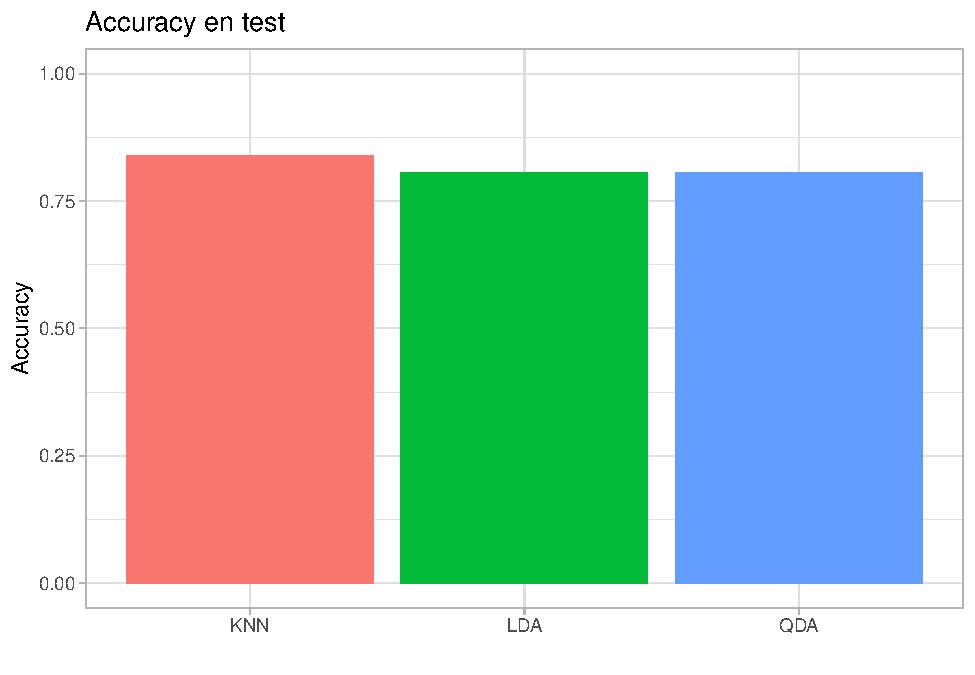
\includegraphics[width=.9\linewidth]{img/Clasificacion_files/figure-latex/unnamed-chunk-33-1}\caption{}\end{figure}

Hacemos notar también que los valores de Kappa son todos bajos, en menor medida para KNN.

\vspace{\baselineskip}

Pese a esto, y ya no solo por tener mejores resultados, sino por no cumplir las asunciones necesarias de obtener resultados de calidad en LDA y QDA, para este problema optaríamos por usar el algoritmo KNN.

A partir de las gráficas 3D de las figuras \ref{3d1} y \ref{3d2} se apreció una difícil separación de las clases, por lo que el algoritmo de vecinos más cercanos nos resulta una aproximación más lógica de entre las utilizadas.

\newpage

\subsubsection{Comparativas generales}

Para comparar la calidad genérica de los algoritmos vamos a aplicar test estadísticos en base a los resultados obtenidos en múltiples datasets.

\vspace{\baselineskip}

Estas son las tablas de resultados que tenemos para test:

\vspace{\baselineskip}

\begin{tabular}{l|r|r|r}
\hline
Dataset & out\_test\_knn & out\_test\_lda & out\_test\_qda\\
\hline
appendicitis & 0.8966667 & 0.8690909 & 0.8109091\\
\hline
australian & 0.6838235 & 0.8579710 & 0.8028986\\
\hline
balance & 0.9024546 & 0.8624101 & 0.9167905\\
\hline
bupa & 0.6865775 & 0.6837924 & 0.5991759\\
\hline
contraceptive & 0.5448653 & 0.5091561 & 0.5173102\\
\hline
haberman & 0.7462069 & 0.7481720 & 0.7512903\\
\hline
hayes-roth & 0.5666667 & 0.5500000 & 0.5875000\\
\hline
heart & 0.6692308 & 0.8481481 & 0.8296296\\
\hline
iris & 0.9642857 & 0.9800000 & 0.9733333\\
\hline
led7digit & 0.7510204 & 0.7420000 & 0.6975000\\
\hline
mammographic & 0.7977698 & 0.8241269 & 0.8194042\\
\hline
monk-2 & 0.9743632 & 0.7703433 & 0.9235535\\
\hline
newthyroid & 0.9071429 & 0.9164502 & 0.9629870\\
\hline
pima & 0.7348861 & 0.7709930 & 0.7412403\\
\hline
tae & 0.3838095 & 0.5245833 & 0.5425000\\
\hline
titanic & 0.7850353 & 0.7760304 & 0.7733032\\
\hline
vehicle & 0.6291452 & 0.7813305 & 0.8522409\\
\hline
vowel & 0.6428571 & 0.6030303 & 0.9191919\\
\hline
wine & 0.6959559 & 0.9944444 & 0.9888889\\
\hline
wisconsin & 0.9735023 & 0.9592185 & 0.9519476\\
\hline
\end{tabular}

\vspace{\baselineskip}
\vspace{\baselineskip}

Comenzamos aplicamos el test de Wilcoxon a cada pareja de algoritmos:

\vspace{\baselineskip}

\textbf{LDA vs QDA:} Obtenemos un ranking de 144 para LDA y 96 para QDA, con un p-value de 0.75 (o nivel de confianza del 25\%).
\begin{verbatim}
V = 96, p-value = 0.7562
alternative hypothesis: true location shift is not equal to 0

  V    V
114 - 96 
\end{verbatim}

Esto nos dice que LDA obtiene mejores resultados pero puesto que el p-value es extremadamente grande no podemos afirmar con garantía estadística que las diferencias entre los tests sean notorias.

\newpage

\textbf{LDA vs KNN:} Ahora obtenemos un ranking de 90 para LDA y 120 para QDA, con un p-value de 0.59 (o nivel de confianza del 41\%).
\begin{verbatim}
V = 120, p-value = 0.5958
alternative hypothesis: true location shift is not equal to 0

 V     V
90 - 120 
\end{verbatim}

Seguimos teniendo un p-value demasiado grande para poder asegurar la diferencia.

\vspace{\baselineskip}

\textbf{QDA vs KNN:} Por último tenemos un ranking de 69 para LDA y 141 para KNN, con un p-value de 0.18 (o nivel de confianza del 82\%).
\begin{verbatim}
V = 141, p-value = 0.1893
alternative hypothesis: true location shift is not equal to 0

 V    V
69 - 141
\end{verbatim}

Aunque buscaríamos al menos un 95\% de confianza, podríamos afirmar al 82\% que los resultados de ambos algoritmos sí son significativamente diferentes.

\vspace{\baselineskip}
\vspace{\baselineskip}

Una comparativa múltiple de los tres algoritmos con el test de \textbf{Friedman} es la siguiente:

\begin{verbatim}
Friedman rank sum test
Friedman chi-squared = 0.7, 
                  df = 2, 
             p-value = 0.7047
\end{verbatim}

El p-value es mayor que 0.05 por lo que no podemos concluir que haya al menos un par de algoritmos de calidad diferente.

\vspace{\baselineskip}
\vspace{\baselineskip}

Aunque el resultado del test de Friedman ya nos indica que un análisis post-hoc es innecesario, puesto que los resultados que se obtengan no van a asegurar la diferencia en la calidad de los algoritmos, por completitud en la memoria aplicamos el post-hoc de \textbf{Holm}:

\begin{verbatim}
1 = KNN, 2 = LDA, 3 = QDA

Pairwise comparisons using Wilcoxon signed rank exact test 

1    2   
2 1.00 -   
3 0.53 1.00
    
P value adjustment method: holm 
\end{verbatim}

Vemos que los p-value son lo más altos posibles, por lo que carece de sentido intentar diferenciar los algoritmos. Aunque podemos notar, tal y como habíamos visto en los test de Wilcoxon, que la diferencia KNN-QDA probablemente sea mayor que el resto de parejas.